\documentclass[a4paper,12pt]{article}
\usepackage[utf8]{inputenc} % utf8 c'est la norme
%\usepackage[applemac]{inputenc}

\usepackage[frenchb]{babel}
\usepackage{graphicx}
\usepackage{float}


\usepackage[top=2.5cm, bottom=2.5cm, left=2.5cm, right=2.5cm]{geometry}

\usepackage[pdfauthor={Agathe Oddon, Jean-Michel Tozzini},%
pdftitle={LO21 : Rapport de projets},%
pagebackref=true,%
pdftex,%
linkcolor=blue,%
colorlinks]{hyperref}

\begin{document}
\title{LO21 : Rapport de projet \\ Calculatrice à notation polonaise inversée}
\author{Agathe \textsc{Oddon} \\ Jean-Michel \textsc{Tozzini}}
\date{Printemps 2012}

\maketitle

\section*{Introduction}
Dans le cadre de notre UV LO21, nous devions réaliser la conception puis implémenter en C++ une calculatrice à notation polonaire inversée.

Le rendu final du projet est composé du présent rapport, du code du programme ainsi que de sa documentation Doxygen.

\tableofcontents

\section{Conception}

	\subsection{Diagramme de classes}
		\begin{figure}[H]
			\center
			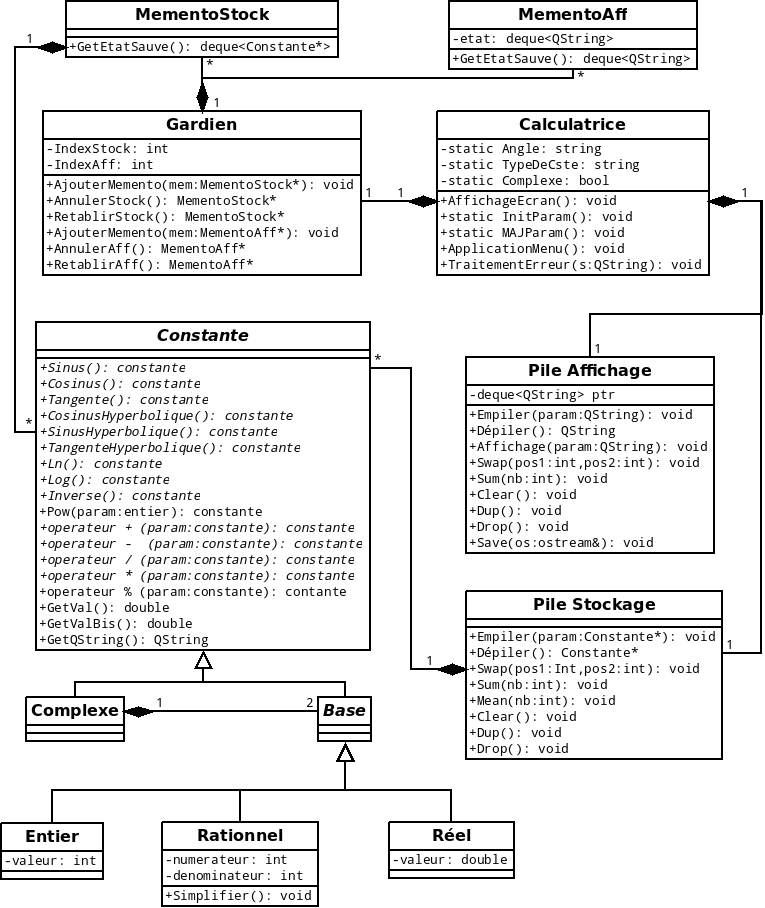
\includegraphics[width=16cm]{UMLProjetLO21v3.png}
			\caption{Diagramme de classe de la Calculatrice à notation polonaise inversée}
		\end{figure}
		
		\subsubsection{Types de données}
			\paragraph{}Nous avons choisi de représenter les données manipulées par la calculatrice comme des objets de trois classes : Entier, Réel, Rationnel, Complexe et Expression. 

			\paragraph{}La classe complexe est composée de deux objets de type Base, classe abstraite de laquelle dérivent Entier, Réel et Rationnel. Cela permet d'obtenir des complexes composés de deux attributs de types différents.

			\paragraph{}Les classes Base, Complexe et Expression dérivent de la classe abstraite et exclusive Constante. 

			\paragraph{}L'utilisation de la classe mère abstraite Constante nous permet à la fois d'empiler des objets de type pointeur sur Constante, et de définir des méthodes polymorphes pour les opérateurs. 

		\subsubsection{Sauvegarde de l'historique}
	 		\paragraph{}L'historique est représenté par les classes Gardiens, mementoAff et mementoStock. Sont utilisation est explicité par la suite.
		\subsubsection{Piles}
			\paragraph{} La pile est géré par deux structures, la pile de stockage qui contient des Constantes et la pile d'affichage qui contient l'équivalent de la pile de stockage mais en QString.
		
		\subsubsection{Calculatrice}
			\paragraph{}Cette classe est la classe princiaple de notre UML, elle gère l'interface graphique ainsi que l'affichage des objets. Elle ne manipule pas directement des données mais par soit par le Gardien pour les mementos soit par les piles pour les constantes et les chaines de caractères associées à ces constantes.

	\subsection{Diagrammes de séquences}
		\begin{figure}[H]
			\center
			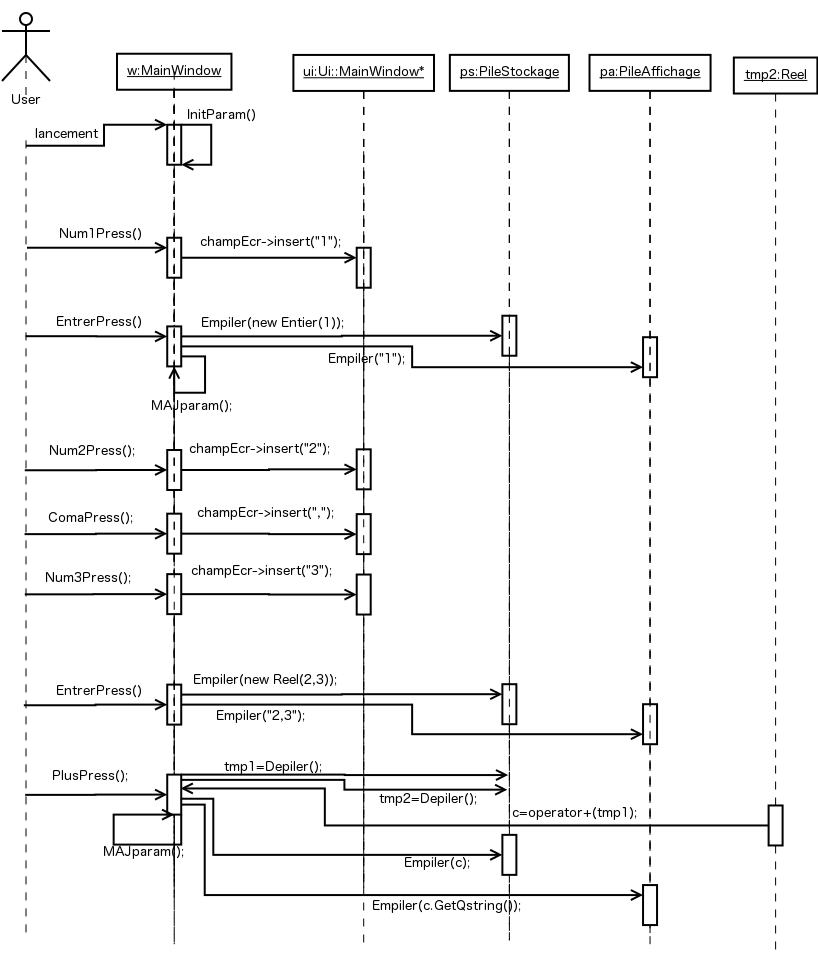
\includegraphics[width=16cm]{diag_seq_1.png}
			\caption{Diagramme de séquence décrivant le lancement de la fenêtre, la saisie de "1", "2,3" , l'appui sur le bouton "+" par l'utilisateur, puis l'addition des deux valeurs.}
		\end{figure}

		\begin{figure}[H]
			\center
			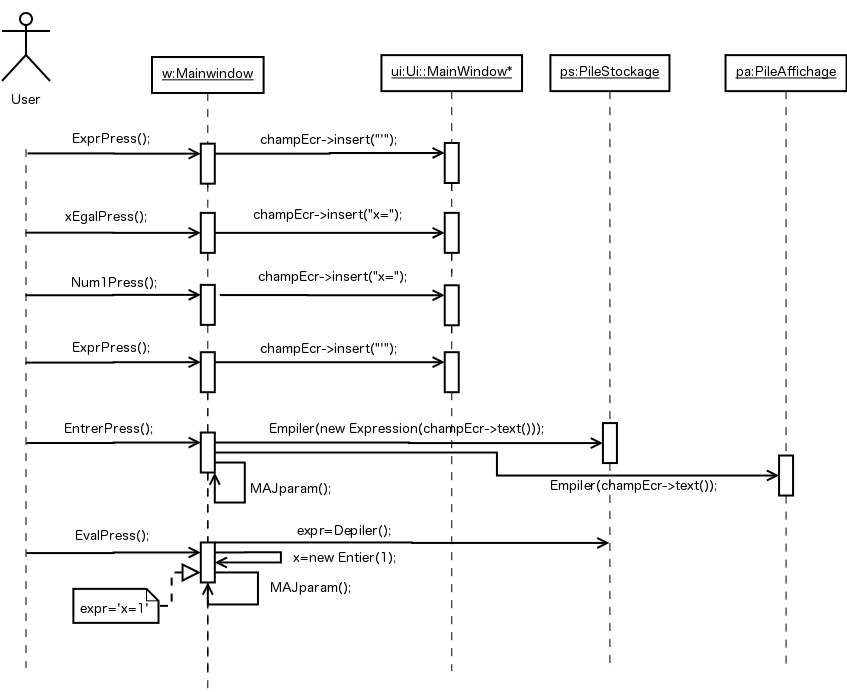
\includegraphics[width=16cm]{diag_seq_2.png}
			\caption{Diagramme de séquence décrivant le lancement de la fenêtre, la saisie de 'x=1', puis l'évaluation de l'expression et la sauvegarde de la valeur 1 dans la variable x.}
			\label{Diagramme sequence x}
		\end{figure}

\section{Implémentation}

	\subsection{Paramètres utilisateur}
		\paragraph{}L'utilisateur dispose d'un menu "Paramètres" lui permettant :
		\begin{itemize}
			\item{De changer le type de constante}
			\item{D'activer ou désactiver le clavier}
			\item{D'activer ou désactiver le mode complexe}
			\item{De choisir l'unité d'angle pour les fonctions cos, sin, tan, cosh, sinh et tanh}
		\end{itemize}
		
		\paragraph{}Le type de constante à été implementé pour une évolution future possible. Ainsi nous avons choisi de garder le type le plus riche en résultat d'une opération et donc de ne pas tenir compte de ce menu.

	\subsection{Variable utilisateur}
		\paragraph{}L'initialisation de la variable utilisateur x se fait par l'intermédiaire d'une expression de la forme 'x=valeur'. Après évaluation (bouton "Eval"), cette expression initialise la variable x avec la valeur spécifiée, qui peut-être de type Entier, Rationnel, Réel ou Complexe. Ce comportement est décrit dans la figure \ref{Diagramme sequence x}.

		\paragraph{}La variable x sera ensuite accessible en tapant directement x ou par l'intermédiaire du bouton "x".

	\subsection{Sauvegarde et restauration de contexte}
		\paragraph{}A l'ouverture du programme, une méthode est lancée permettant la restauration du contexte de la Calculatrice : il s'agit des piles, des valeurs des menu et de la valeur de la variable utilisateur si elle a été initialisée. Cette méthode interroge un fichier "param.txt" contenant les données du contexte. Si il s'agit de la première ouverture du programme, le fichier est initialisé avec des valeurs par défaut.

		\paragraph{}A chaque entrée de l'utilisateur ou modification des paramètres, une méthode est lancée pour mettre à jour le ficher.

	\subsection{Historique}
		\paragraph{}Notre historique est implémenté avec le design pattern memento. Ainsi il est composé de trois classe, le Memento qui est une version de sauvegarde, le gardien qui est composé de plusieurs mementos et la pile est l'élément à sauvegarder. 
		
		 \paragraph{}Lors d’un changement de la pile, un memento est crée pour chacune des deux piles. Ce memento est une copie de la pile, Il est ensuite empilé dans le gardien. Les fonctions annuler et rétablir naviguent dans les mementos du gardien pour récupérer ces mémentos et utilise une méthode des pile pour lire et récupérer l'information contenu dans le memento.
		 
	\subsection{Exceptions}
		\paragraph{}Nous avons choisi d'implémenter qu'une seule classe Exception. Cette classe est composé d'une chaine de caratères et d'une méthode renvoyant celle-ci. Lors de l'execution d'un \emph{throw} une instance d'erreur est créée et la chaine de caractère est envoyé par la méthode de la classe Exception. Cette chaine de caractère est ensuite prise en charge par une méthode de la calculatrice pour l'affichage dans l'ecran prévu à cet effet.
		
	\subsection{Méthodes de Constante et ses classes filles}
		\paragraph{}Pour les opérateurs utilisables avec plusieurs types de données, par exemple l'opérateur + peut-être utilisés avec les types Entier, Réel, Rationnel, Complexe et Expression, nous avons d'abord défini une méthode de Constante permettant d'appeler la bonne méthode de ses classes filles.

		\paragraph{}Toutes les méthodes ont ensuite dues être implémentées pour tous les types de données. Nous avons fait le choix de toujours renvoyer le type le plus riche. Par exemple, l'addition d'un entier et d'un réel renverra toujours un réel, de même la soustraction d'un rationnel et d'un complexe renverra un complexe.\footnote{Pour les opérations entre les types Rationnel et Réel, nous avons choisi de toujours renvoyer un Réel, méme si il ne s'agit pas du type le plus riche, du fait que nous ne pouvons pas convertir un Réel en Rationnel sans perdre d'information sur celui-ci.} Les méthodes qui n'acceptait pas le type de données, par exemple l'opérateur mod (modulo) n'accepte que les entiers, renvoient des exceptions.

\end{document}
